% The evaluation's two figures of the CIRP CMS 2026 paper, for section 4. Draft of 1 Nov 2026.
%
% Drawn by cell/eval/figures.py from the newest results in cell/eval/results (effort of 29 Oct;
% scenarios of 29 Oct, five runs each, medians). Each one column wide. The module's drawing is a page
% of docs/figures/cirp-figures.drawio; its photo goes into figures/filling-module-photo.jpg, numbered
% as the drawing is.
%
% The evaluation is being rethought (docs/paper-outline.md, section 4): effort and downtime may go.

\begin{figure}[t]
  \centering
  \begin{minipage}[b]{0.48\columnwidth}
    \centering
    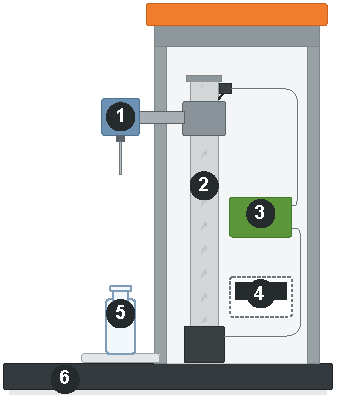
\includegraphics[width=\linewidth]{figures/filling-module.pdf}\\[2pt]
    (a)
  \end{minipage}\hfill
  \begin{minipage}[b]{0.48\columnwidth}
    \centering
    \IfFileExists{figures/filling-module-photo.jpg}{%
      \includegraphics[width=\linewidth]{figures/filling-module-photo.jpg}}{%
      \fbox{\parbox[c][1.1\linewidth][c]{0.9\linewidth}{\centering photo to come}}}\\[2pt]
    (b)
  \end{minipage}
  \caption{The filling module, (a)~drawn and (b)~as built: (1)~pump, (2)~linear axis with a stepper
    motor, (3)~Raspberry Pi~5 running 4diac FORTE, (4)~scale (simulated), (5)~vial on a shuttle of
    (6)~the planar motor table.}
  \label{fig:module}
\end{figure}

\begin{figure}[t]
  \centering
  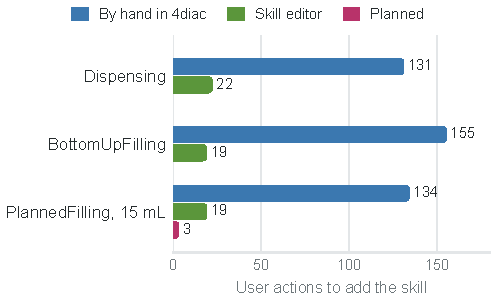
\includegraphics[width=\columnwidth]{figures/effort.pdf}
  \caption{The engineering effort of a new composite skill on the filling module, in user actions
    counted as in~\cite{dorofeev2021orchestrator}: by hand in 4diac, in the skill editor on the AAS,
    and planned, where only the requirement is entered.}
  \label{fig:effort}
\end{figure}

\begin{figure}[t]
  \centering
  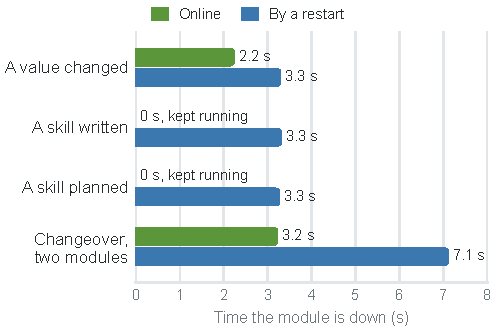
\includegraphics[width=\columnwidth]{figures/downtime.pdf}
  \caption{How long the module is down for each change, made online by the reconciler and by a new
    boot file and a restart; FORTE on a PC with simulated IO, medians of five runs. A new skill,
    written or planned, is created while another skill keeps running. For a changed value the module
    leaves Execute and returns to it. In the changeover of two modules, the stoppering module does
    so for its value.}
  \label{fig:downtime}
\end{figure}
